\chapter{Experiments}
\label{sec:experiments}
This chapter describes the experiments that have been done on SMDP Q-learning,
O-MCTS and OL-MCTS. The algorithms are compared to the Monte Carlo tree search
algorithm, as described in Section \ref{subsec:mcts}. The learning capacities of
SMDP Q-learning and OL-MCTS are demonstrated by experimenting with the toy
problem, \textit{prey}. Furthermore, all algorithms are run on a set of
twenty-eight different games in the VGDL framework. The set consists of all the
games from the first four training sets of the GVGAI competition, excluding
puzzle games that can be solved by an exhaustive search and have no random
component (e.g. NPCs). The games have 5 levels each, the first of which
traditionally is the easiest and the last of which is the hardest.

Firstly, this chapter demonstrates the performance of our implementation of SMDP
Q-learning. Secondly, we compare O-MCTS to MCTS, by showing the win ratio and
mean score of both algorithms on all the games. Then, we show the improvement
that OL-MCTS makes compared to O-MCTS if it is allowed 4 games of learning time.
We demonstrate the progress it achieves by showing the first and last of the
games it plays.  Lastly we compare the three algorithms by summing over all the
victories of all the levels of each game.  Following the GVGAI competition's
scoring method, algorithms are primarily judged on their ability to win the
games. The scores they achieve are treated as a secondary objective.

\section{Game Test Set}
\label{subsec:games}
The algorithms we propose are tested on a subset of the first four training sets
of the GVGAI competition. We exclude puzzle games that can be solved by an
exhaustive search, because the algorithms will not be able to benefit from the
option set that was constructed for these experiments, since the games have no
random components. This leaves us with the twenty-eight games that are described
in this section. All games the game have a time limit of 2000 time steps, after
which the game is lost unless specified otherwise.

The games are described in decreasing order of the performance of a random
algorithm, an algorithm that always chooses a random action, as an indication of
the complexity of the games. The graphs in the experiments have the same
ordering.

\begin{enumerate}
	\item Surround: 
		The aim of the game is to walk as far as possible. You get a point for
		every move you are able to make and afterwards, a non-traversable sprite
		is added in your previous location. The game is ended, and won, by using
		the \texttt{use} action. An NPC is doing the same as you and kills you
		on contact.
	\item Infection:
		The aim of the game is to infect as many healthy (green) animals (NPCs)
		as possible, by colliding with a bug or infected animal first, and then
		with a healthy animal. When animals collide with other infected animals,
		they get infected as well. Blue sprites are medics that cure infected
		animals and the avatar, but can be killed with the avatar's sword. The
		player wins when every animal is infected.
	\item Butterflies: 
		The avatar hunts butterflies, the avatar wins if he has caught (walked
		into) all of them. Butterflies spawn at certain locations, so sometimes
		waiting longer to end the game can increase the eventual score.
	\item Missile Command: 
		Missiles move towards some city-sprites that need to be defended by the
		avatar. The avatar can destroy missiles before they reach the city by
		standing next to a missile and using his weapon. When all missiles are
		gone and some of the city sprites are still left, the game is won. If
		all the city sprites are gone, the game is lost.
	\item Whackamole:
		The avatar must collect moles that appear at holes. The enemy player is
		doing the same. The player wins after 500 time steps, but loses if it
		collides with the enemy.
	\item Aliens:
		Based on the commonly known game \textit{space invaders}. Aliens appear
		at the top of the screen. The avatar can move left or right and shoot
		missiles at them. The avatar loses when the aliens reach the bottom and
		wins when all the aliens are dead. The avatar should evade the aliens'
		missiles as well.
	\item Plaque attack:
		Hamburgers and hot dogs attack teeth that are spread over the screen. The
		avatar must shoot them with a projectile weapon in order to save at
		least one tooth. The avatar can repair damaged teeth by walking into
		them. The game is won if all the food is gone and lost if the teeth are
		gone.
	\item Plants:
		Emulating the \textit{Plants vs. Zombies} game, the avatar should plant
		plants that shoot peas at incoming zombies. The zombies can kill the
		plants by shooting back. The avatar wins when the time runs out, but
		loses when a zombie reaches the avatar's defensive field.
	\item Bait: 
		The avatar should collect a key and walk towards a goal. Holes in the
		ground kill the avatar when he moves into them, but can be closed by
		pushing boxes into them (after which both the hole and the box
		disappear). By collecting mushrooms, the player can get more points.
	\item Camel Race:
		The avatar must get to the finish line before any other camel does.
	\item Survive Zombies:
		The avatar should evade the zombies that walk towards him. When a zombie
		touches a bee, it drops honey. The avatar can pick up honey in order to
		survive one zombie attack. When a zombie touches honey, it dies. If the
		avatar survives for 1000 time steps, it wins the game.
	\item Seaquest:
		The avatar can be killed by animals, or kill them by shooting them. The
		aim is to  rescue divers by taking them to the surface. The avatar can
		run out of oxygen, so it must return to the surface every now and then.
		The game is won after 1000 time steps, or lost if the avatar dies.
	\item Jaws:
		The avatar must shoot dangerous fish that appear from portals to collect
		the resources they drop.  A shark appears at a random point in time,
		that can not be killed by shooting, but can be killed by touch, given
		that the avatar has enough resources. If he has too little resources,
		the game is lost. Otherwise, after 1000 time steps, the game is won.
	\item Firestorms:
		The avatar must avoid flames while traversing towards the exit. He can
		collect water in order to survive hits by flames, but the game is lost
		if a flame hits the avatar when he has no water. 
	\item Lemmings:
		Lemmings are spawned from a door and try to get to the exit. The avatar
		must destroy their obstacles. There are traps that have to be evaded by
		the avatar and the lemmings. The game is won when all the lemmings are
		gone, or lost when the avatar dies.
	\item Firecaster:
		The avatar must burn wooden boxes that obstruct his path to the exit.
		The avatar needs to collect ammunition in order to be able to shoot.
		Flames spread, being able to destroy more than one box, but the avatar
		should evade them as well. When the player's health reaches 0 he loses,
		but when he reaches the exit he wins.
	\item Pacman:
		The avatar must clear the maze by eating all the dots, fruit pieces and
		power pills.  When the player collides with a ghost he is killed,
		unless he has eaten a power pill recently.
	\item Overload:
		The avatar must collect a determined number of coins before he is
		allowed to enter the exit. If the avatar collects more coins than that,
		he is trapped, but can kill marsh sprites with his sword for points.
	\item Boulderdash:
		The player collects diamonds while digging through a cave. He should
		avoid boulders that fall from above and avoid or kill monsters. If the
		avatar has enough diamonds, he may enter the exit and wins.
	\item Zelda:
		The avatar should collect a key and walk towards the door in order to
		win. He can kill monsters with his sword for additional points, but the
		monsters kill the avatar on touch.
	\item Chase:
		The avatar chases and kills goats that are scared. However, when a
		scared ghost walks into the carcass of one of the others, he becomes
		angry and capable of killing the avatar. When there are no scared goats
		left, the avatar wins.
	\item Digdug:
		The aim of the game is to collect all the gems and gold coins by digging
		a way through a cave. Enemies kill the player on collision. When the
		avatar presses \textsc{use} in two consecutive time steps, it shoots a boulder to
		kill the enemy.
	\item Bolo Adventures:
		The avatar should reach the goal. He can push around boxes 1 cell at a
		time, or boulders that roll until they hit another obstacle. Boulders
		can fill holes that obstruct the player's movement, and both boulders
		and boxes can block laser beams that kill the avatar.
	\item Roguelike:
		The avatar should escape a maze through the door. There are monsters
		that can be killed with a sword, after it has been picked up. Doors can
		be opened with keys. Extra points are awarded for picking up gold and
		gems. After being hit by an enemy, it is possible to exchange gold for
		health.
	\item Boulderchase:
		Similar to \textit{boulderdash}, but enemies drop diamonds when they are
		killed and they can dig paths through the cave, like the player.
	\item Eggomania:
		A chicken at the top of the screen throws eggs. The aim of the game is
		to move from left to right in order to catch the eggs. If the avatar
		fails to catch even one, the game is lost. When the avatar
		has collected enough eggs, it is possible to shoot the chicken to win
		the game.
	\item Portals:
		The avatar needs to find the exit of the maze. He can use the available
		portals to teleport from one place to another. The aim of the game is to
		find the correct sequence of portals that lead to the exit. There are
		moving objects that kill the player on touch.
	\item Frogs:
		Commonly known as \textit{frogger}, the avatar is a frog, that needs to
		cross a busy road and a river. On the road, the frog should evade the
		trucks that move by. On the river, the frog should leap from tree trunk
		to tree trunk in order to reach the exit.
\end{enumerate}

We apply Monte Carlo tree search to this set of games as our baseline algorithm.
Furthermore, we run SMDP Q-learning, O-MCTS and OL-MCTS.  The GVGAI competition
comes with some predefined competition parameters: every algorithm has a maximum
of one second to initialize, before starting the game. Then, the algorithm has a
maximum of forty milliseconds per time step to return an action, after which a
new game state is given. If the agent exceeds the time limit, the action
\textsc{null} will be applied and the avatar will not do anything\footnote{There
	seems to be a bug in the system, that causes actions to sometimes take
	hundreds of milliseconds to simulate. This bug has been reported to the
	competition's discussion platform by several users. Because this bug was not
	solved at the time of writing, we chose to not honor the GVGAI competition's
	original rule to disqualify a controller that does not return an action
within fifty milliseconds.}. To enable inter-game learning, the framework is
edited to be able to pass information from one game to the next. After a game is
finished, the learning algorithms OL-MCTS and SMDP Q-learning get the
possibility to save their values to a file. The file can be read during the
initialization of the next game. Since the initialization has a time limit, the
algorithms are encouraged to minimize their file size.

We empirically optimize the parameters of the O(L)-MCTS algorithm for these
experiments. We use discount factor $\gamma = 0.9$. The maximum search depth $d$
is set to 70, which is higher than most alternative tree search algorithms, for
example in the GVGAI competition, use. The number of node visits after which
\textsf{uct} is used, $v$, is set to 40. Crazy stone parameter $K$ is set to
$2.5$. The maximum search depth for MCTS is set to 10, which is value the GVGAI
implementation uses by default.  MCTS and O-MCTS have \textsf{uct} constant $C_p
= \sqrt{2}$. SMDP Q-learning has a maximum exploration depth $d$ of 20, an
exploration parameter $\varepsilon$ of 0.2 and $\alpha$ is set to $0.1$.  All the
experiments are run on an Intel %\textsuperscript{\textregistered} 
Core %\texttrademark 
i7-2600, 3.40GHz quad core processor with 6 GB of DDR3, 1333 MHz RAM memory. In
all the following experiments on this game set, each algorithm plays each of the
5 levels of every game 20 times. 

\section{SMDP Q-learning}
\label{subsec:experiments-smdp-qlearning}
In this section, the SMDP Q-learning implementation that was proposed in chapter
\ref{subsec:smdp-qlearning-gvgp} is tested. Q-learning's first implementation
requirement is a serialization of the state space.  Furthermore, to prevent the
Q-table to become too big we apply a state space reduction similar to that of
other GVGAI learning algorithms \cite{samothrakis2015neuroevolution}.  The
following values are saved:

\begin{itemize}
	\item the avatar orientation;
	\item the avatar's resources (one or more quantities, e.g.,
		\texttt{"diamonds:3"});
	\item the direction and Euclidean distance to the nearest:
		\begin{itemize}
			\item NPC,
			\item other movable sprite,
			\item resource,
			\item portal,
			\item other immovable sprite.
		\end{itemize}
\end{itemize}

Although with this representation information about the map and the grid
location of the avatar is lost, it enables the algorithm to keep a smaller and
more generalized Q-table. As a result, it can work on more games without running
out of memory.

\begin{figure}
	\centering
	\subfigure[Win ratio on \textit{prey}]{
		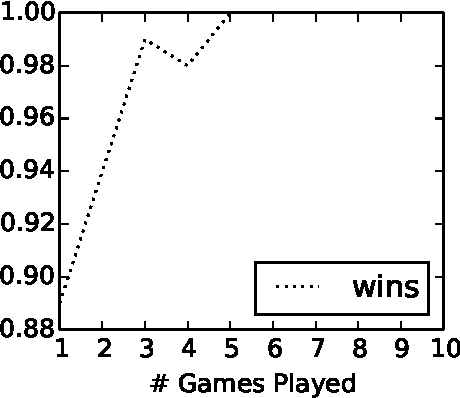
\includegraphics[scale=.61]{includes/winsQlearningPrey-crop}
		\label{fig:wins-qlearning-prey}
	}
	\subfigure[Time taken for \textit{prey}]{
		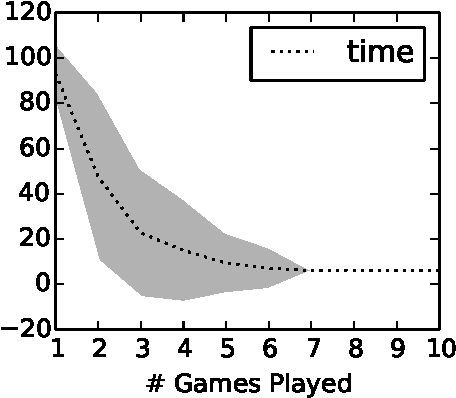
\includegraphics[scale=.61]{includes/timeQlearningPrey-crop}
		\label{fig:time-qlearning-prey}
	}
	\caption{Mean performance over 100 times 10 games of Q-learning the
	\textit{prey} toy problem.}
	\label{fig:qlearning}
\end{figure}

The first experiment is a proof of concept of our implementation of SMDP
Q-learning with our option set and state space reduction. We apply the algorithm to the
first level of the toy problem, \textit{prey}. The results can be seen in figure
\ref{fig:qlearning}. We can see that the algorithm wins consistently starting
from the fifth game The time it takes to win converges to 6, which is
the least number of steps possible to reach the prey. We can conclude that it
wins consistently by applying the correct options. This indicates that the
values for the Q-table converge to their optima. Unfortunately, when applied to
the second level of \textit{prey}, which requires a more complex and longer
action sequence, SMDP Q-learning is not able to find a winning policy in the
first 500 games, after which its Q-table becomes too large to load in the
initialization time and the algorithm is disqualified.

\begin{figure}
	\centering
	\makebox[\columnwidth]{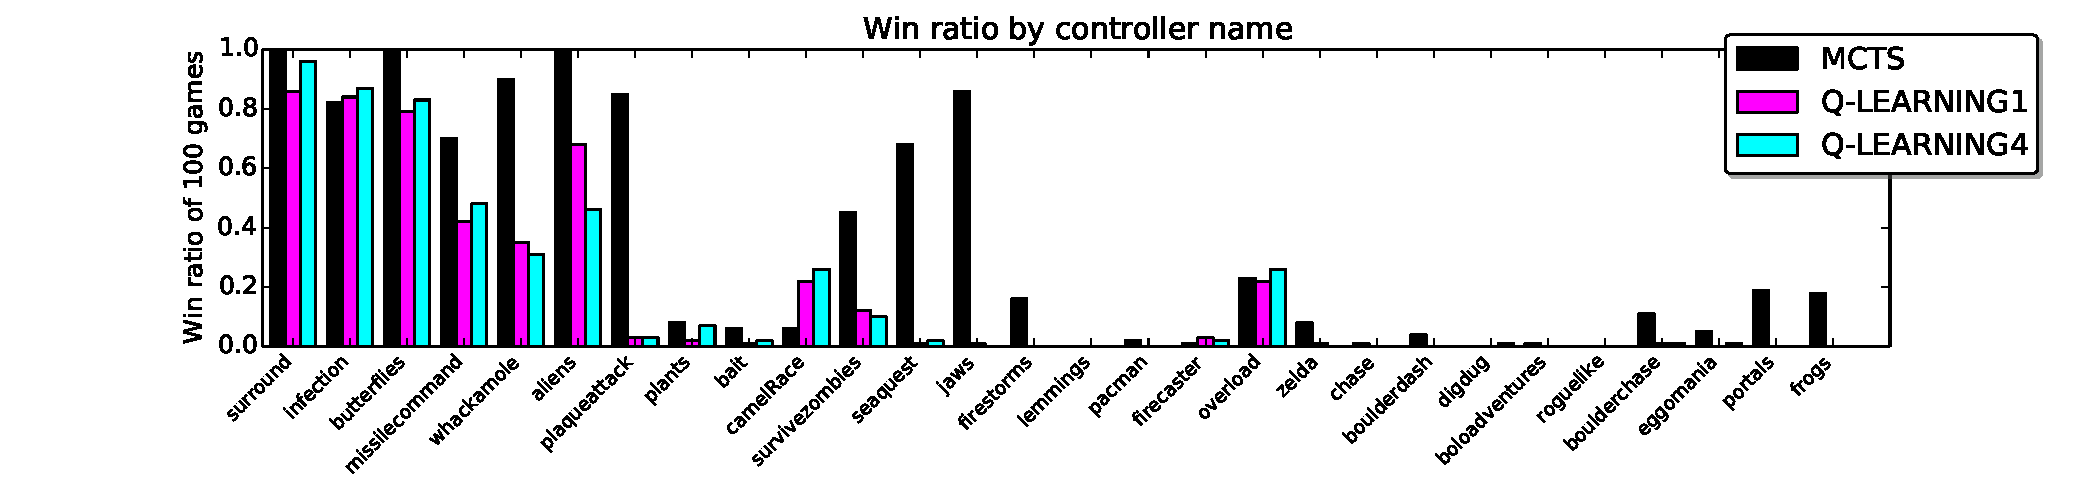
\includegraphics[width=1.25\textwidth]{includes/qLearningWins}}
	\vspace{-.8cm}
	\caption{Win ratio of SMDP Q-learning per game on all levels, compared to Monte Carlo Tree Search.}
	\label{fig:qlearning-wins}
	\centering
	\makebox[\columnwidth]{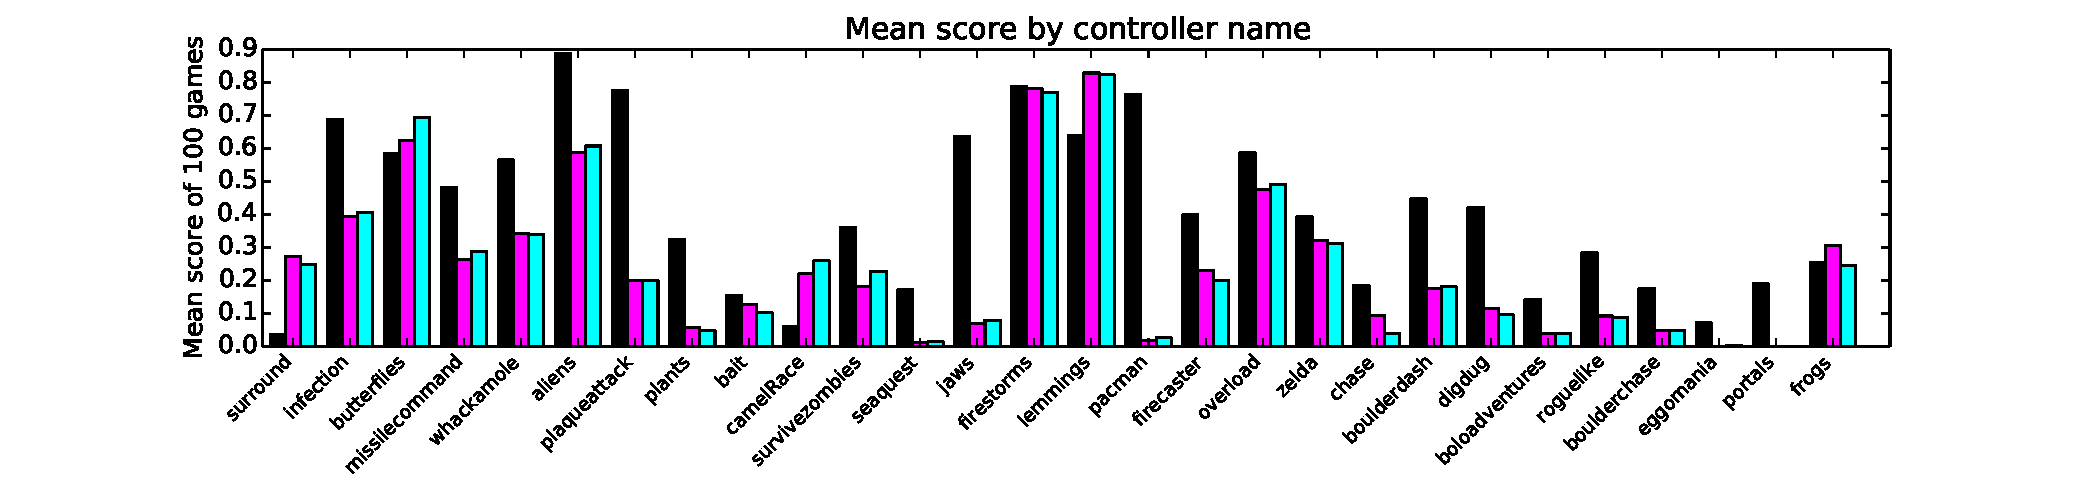
\includegraphics[width=1.25\textwidth]{includes/qLearningScores}}
	\vspace{-.8cm}
	\caption{Mean normalized score of the algorithms per game 1 means the
	highest score achieved by all the algorithms (including all of the following
tests), 0 the lowest.}
	\label{fig:qlearning-scores}
\end{figure}

For the next experiment, SMDP Q-learning and Monte Carlo tree search are applied
to all the games described in Chapter \ref{subsec:games}. The results are shown
in Figures \ref{fig:qlearning-wins} and \ref{fig:qlearning-scores}. The scores
in Figure \ref{fig:qlearning-scores} are normalized using the data of all the
algorithms, including O-MCTS and OL-MCTS and the random algorithm. The best
score achieved by any of the algorithms in a level of a game is 1, the worst is
normalized to 0. Like the game descriptions in Section \ref{subsec:games}, the
bars are ordered by the performance of the random algorithm. From left to right
its win ratio and score decreases, from which we can assume that the leftmost
game is the easiest and the rightmost is the hardest.

The bars labeled Q-LEARNING1 show the performance of SMDP Q-learning in
the first game it plays. It is then allowed three subsequent games to learn.
The score of the fourth game is shown by the bars labeled Q-LEARNING4. Our
further experiments have shown that a longer learning sequence decreases the
total score for Q-learning, because the size of the Q-table causes the algorithm
to be disqualified during initialization.

The figures show that MCTS outperforms SMDP Q-learning in almost all the games.
Our theory is that if the algorithm is allowed to learn for more games and is
given more time in the initialization phase to load the Q-table, its performance
will increase. However, the framework does not allow this, and the size of the
Q-table might still become infeasible, since the number of states in these
games is many times larger than the type of problem that SMDP Q-learning with
options was demonstrated with \cite{sutton1999between}. For this reason, in the
next section the results of SMDP Q-learning will be omitted and we will compare
O-MCTS to MCTS.

\section{O-MCTS}
This section describes the results of the option Monte Carlo tree search
algorithm in comparison with the standard Monte Carlo tree search algorithm.
This demonstrates the improvement that can be achieved by using our method to
enhance MCTS with our option set.

\label{subsec:omcts}
\begin{figure}
	\centering
	\makebox[\columnwidth]{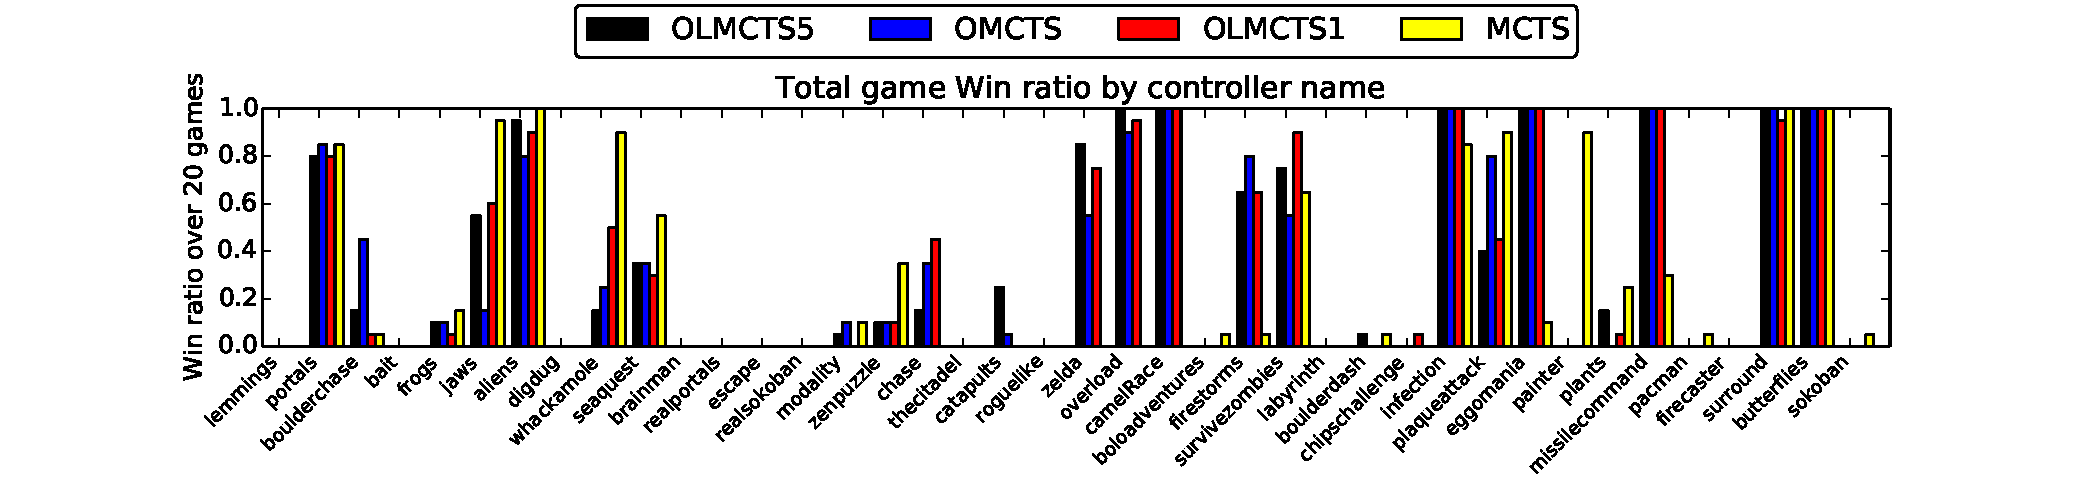
\includegraphics[width=1.25\textwidth]{includes/wins}}
	\vspace{-.8cm}
	\caption{Win ratio of the algorithms per game on all levels.}
	\label{fig:omcts-wins}
	\centering
	\makebox[\columnwidth]{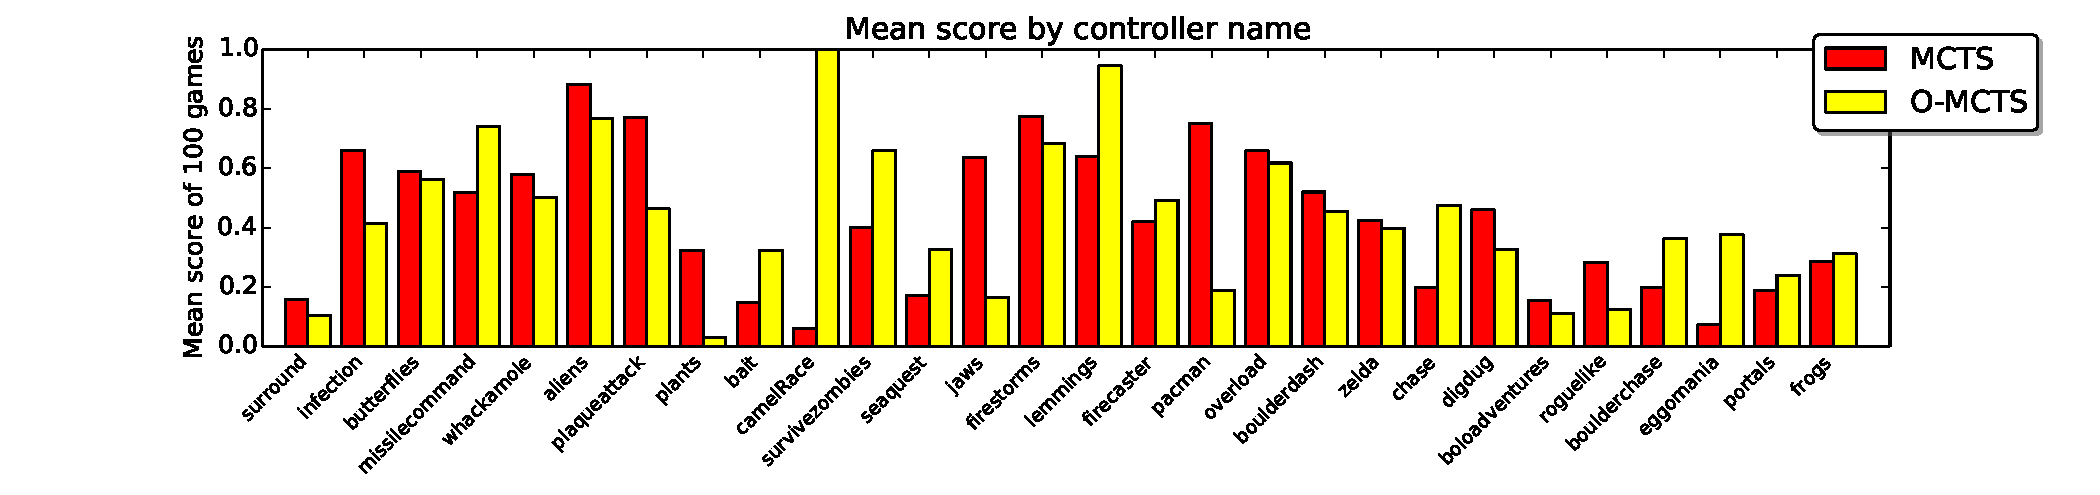
\includegraphics[width=1.25\textwidth]{includes/scores}}
	\vspace{-.8cm}
	\caption{Mean normalized score of the algorithms per game 1 means the
	highest score achieved by all the algoriths, 0 the lowest.}
	\label{fig:omcts-scores}
\end{figure}

Figures \ref{fig:omcts-wins} and \ref{fig:omcts-scores} respectively show the
win ratio and normalized score of the algorithms for each game. In short, the
O-MCTS algorithms performs at least as good as MCTS in almost all games, and
better in most.

O-MCTS outperforms MCTS in the games \textit{missile command}, \textit{bait},
\textit{camel race}, \textit{survive zombies}, \textit{firestorms},
\textit{lemmings}, \textit{firecaster}, \textit{overload}, \textit{zelda},
\textit{chase}, \textit{boulderchase} and \textit{eggomania} winning more games
or achieving a higher mean score. By looking at the algorithm's actions for
these games, we can see that O-MCTS succeeds in efficiently planning paths in a
dangerous environment, enabling it to do a further forward search than the
ordinary Monte Carlo tree search. 
\textit{Camel race} requires the player to
move to the right for 80 consecutive turns to reach the finish line. No
intermediate rewards are given to indicate that the agent is walking in the
right direction. This is hard for MCTS, since it only looks 10 turns ahead.
O-MCTS always wins this game, since it can plan forward a lot further.
Furthermore, the rollouts of the option for walking towards the finish line have
a bigger chance of reaching the finish line than the random rollouts executed by
MCTS. 
In \textit{Overload}, a sword has to be picked up before the avatar can finish the
game, which seems to be too hard for MCTS, but poses less of a problem for
O-MCTS.  Furthermore, in \textit{zelda} we can see that the MCTS algorithm
achieves roughly the same score as O-MCTS, but does not win the game, since
picking up the key and walking towards the door is a difficult action sequence.
We assume that the mean score achieved by MCTS is because it succeeds in killing
the monsters, whereas O-MCTS achieves its score by picking up the key and
walking to the door.  These results indicate that O-MCTS performs better than
MCTS in games where a sequence subgoals have to be reached.

The MCTS algorithm performs better than O-MCTS in \textit{pacman},
\textit{whackamole}, \textit{jaws}, \textit{seaquest} and \textit{plaque attack}
(note that for \textit{seaquest}, O-MCTS has a higher mean score, but wins less
than MCTS). A parallel between these games is that they have a very
big number of different sprites, for each of which several options have to be
created by O-MCTS. When the number of options becomes too big, constructing the
set of possible options $\mathbf{p}_s$ for every state $s$ becomes so
time-consuming that the algorithm has too little time to build a tree and find
the best possible action. To test this hypothesis we increased the computation
time for O-MCTS to 120ms and found that the win ratio of O-MCTS increases to
around $0.8$ for \textit{seaquest} and \textit{plaque attack}, whereas the win
ratio for MCTS increased to $0.9$ and $0.7$ respectively. This means that with
more action time, the difference between O-MCTS and MCTS is reduced for
\textit{seaquest} and O-MCTS outperforms MCTS on \textit{plaque attack}.

\begin{figure}
	\centering
	\subfigure[\textit{Plaque attack}, level 4]{
		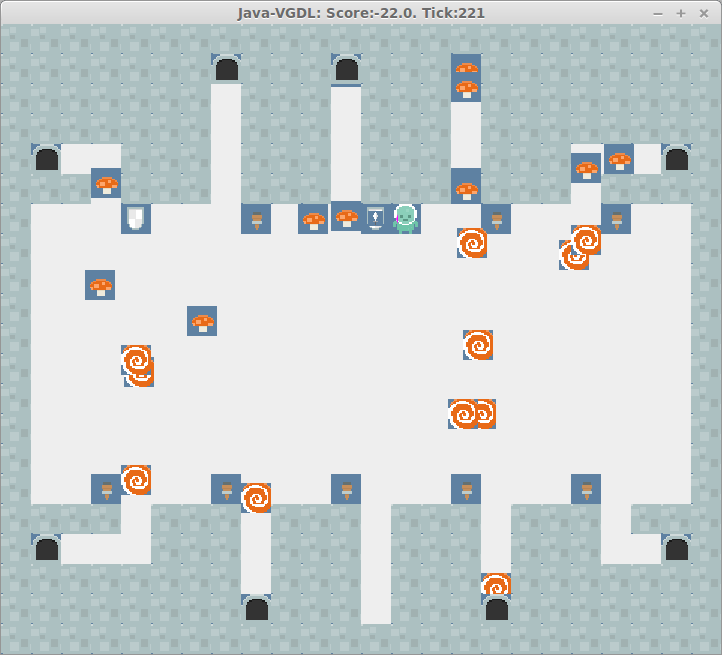
\includegraphics[scale=.2]{includes/plaqueattack}
		\label{fig:plaqueattack}
	}
	\subfigure[\textit{Overload}, level 4]{
		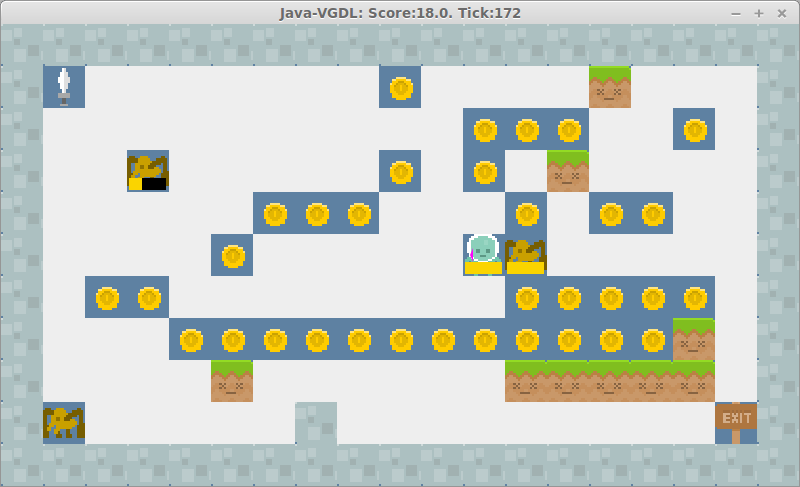
\includegraphics[scale=.2]{includes/overload}
		\label{fig:overload}
	}
	\caption{The different in size of \textit{plaque attack} ($24\times21$) and 
		\textit{overload} ($19\times11$)}
	\label{fig:game-size}
\end{figure}

Another difficulty for O-MCTS in these games is illustrated in figure
\ref{fig:game-size}: the games \textit{seaquest}, \textit{plaque attack} and
\textit{pacman} have very large maps, in which using A Star to calculate routes
becomes increasingly time consuming. For example, \textit{plaque attack}, seen
in Figure \ref{fig:plaqueattack}, has a grid of 24 by 21 blocks, which is more
than twice the size of \textit{overload}, seen in Figure \ref{fig:overload} with
a grid of 19 by 11 blocks.

Lastly, the game \textit{jaws} starts with an almost empty screen. The algorithm
is then inclined to walk towards the portals that are on the screen, because
there are more options that lead towards portals than options that do not. These
portals spawn enemies, which upon spawning immediately kill the avatar. 

In summation, O-MCTS performs good on most games. When it does not, it mostly
struggles with the overhead that is created by maintaining the option set:
planning routes with A Star, checking if options are finished and constructing
the possible option set, $\mathbf{p}_s$. By learning option values, OL-MCTS
should be able to improve performance on these games.

\section{OL-MCTS}
\label{subsec:olmcts}

\begin{figure}
	\centering
	\subfigure[Win ratio on \textit{prey}]{
		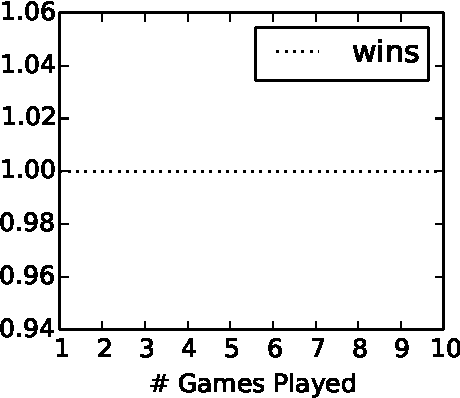
\includegraphics[scale=.61]{includes/winsOlmctsPrey-crop}
		\label{fig:wins-olmcts-prey}
	}
	\subfigure[Time taken for \textit{prey}]{
		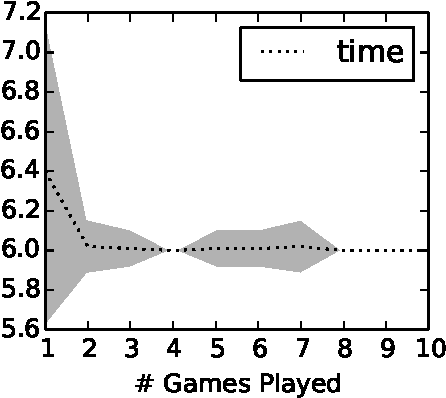
\includegraphics[scale=.61]{includes/timeOlmctsPrey-crop}
		\label{fig:time-olmcts-prey}
	}
	\caption{Mean performance over 100 times 10 games of OL-MCTS on the
	\textit{prey} toy problem.}
	\label{fig:olmctsPrey}
\end{figure}

This section describes the improvements that can be found on the O-MCTS
algorithm, when a bias can be learned towards certain more feasible options. The
improvement that was proposed in Chapter \ref{sec:learning} is compared to
the performance of O-MCTS in this section.

Firstly, by running Option Learning MCTS on the toy problem \textit{prey}, we
demonstrate its capacity to learn, similar to what was done in section
\ref{subsec:experiments-smdp-qlearning}. The results are displayed in Figure
\ref{fig:olmctsPrey}. OL-MCTS never loses the toy problem and after the first
game almost always takes 6 time steps to catch the prey. 

As more challenging test, the algorithm is run on the second level and we set
the maximum rollout distance $d$ to 10, so the prey is outside the reach of the
rollouts. Figure \ref{fig:olmctsPrey3} demonstrates that OL-MCTS successfully
learns to prefer the options that lead to the avatar over the other options.
This results in the algorithm taking a path that is close to the smallest number
of time steps needed starting from game 2, even though in the first ten time
steps, the algorithm has no rollouts that lead to the winning condition. From
this we can conclude that the algorithm is capable to learn from which options
it benefits and bias its search towards those. Furthermore, we observe that the
performance of OL-MCTS is better than that of SMDP Q-learning on the same
problem.

\begin{figure}
	\centering
	\subfigure[Win ratio on \textit{prey} level 2]{
		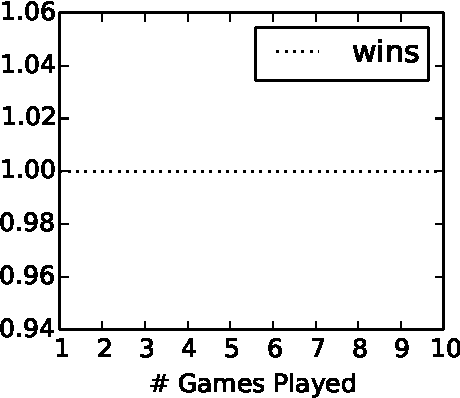
\includegraphics[scale=.61]{includes/winsOlmctsPrey3-crop}
		\label{fig:wins-olmcts-prey3}
	}
	\subfigure[Time taken for \textit{prey} level 2]{
		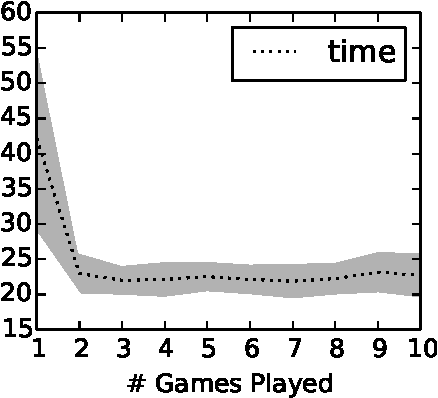
\includegraphics[scale=.61]{includes/timeOlmctsPrey3-crop}
		\label{fig:time-olmcts-prey3}
	}
	\caption{Mean performance over 100 times 10 games of OL-MCTS on the second
		level of the \textit{prey} toy problem.}
	\label{fig:olmctsPrey3}
\end{figure}


\begin{figure}
	\centering
	\makebox[\columnwidth]{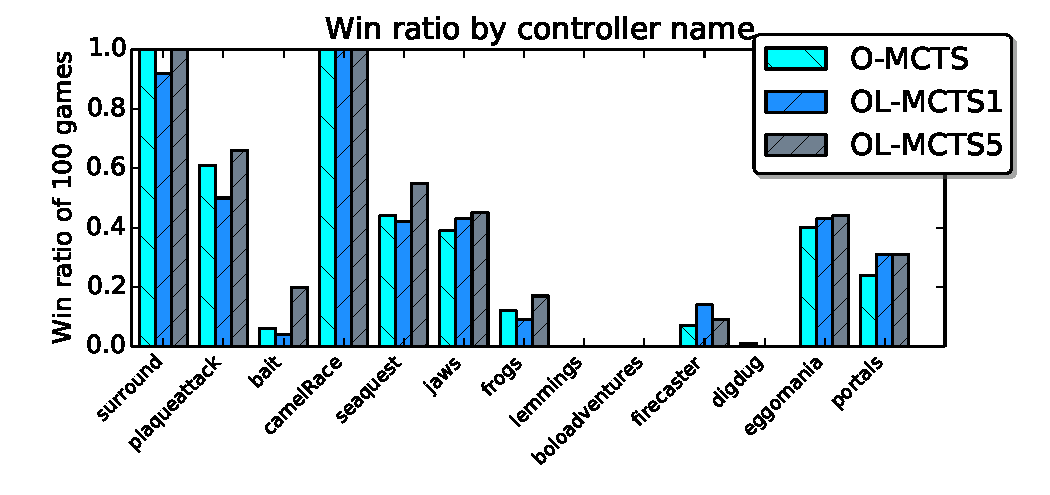
\includegraphics[width=1.25\textwidth]{includes/winsOLMCTS}}
	\vspace{-.8cm}
	\caption{Win ratio of OL-MCTS compared to O-MCTS in its first and fifth game.}
	\label{fig:wins-olmcts}
	\centering
	\makebox[\columnwidth]{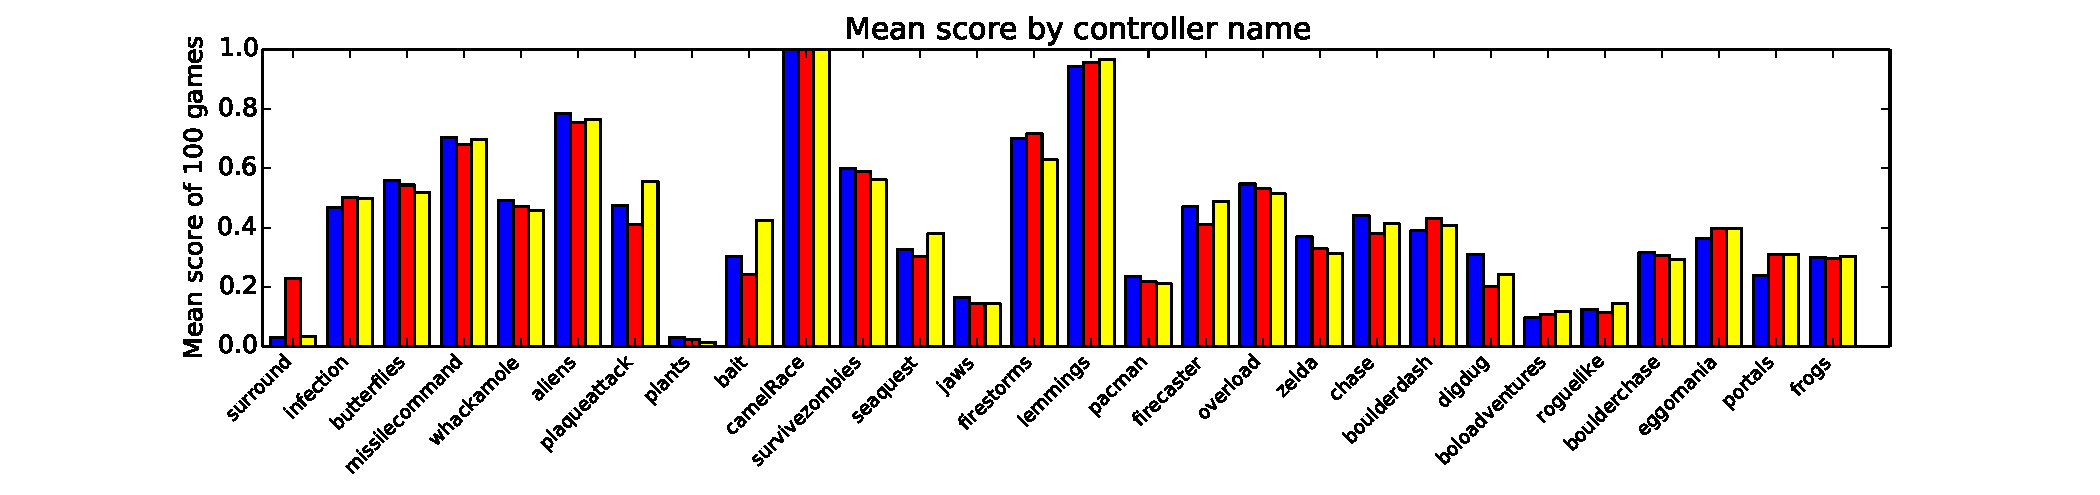
\includegraphics[width=1.25\textwidth]{includes/scoresOLMCTS}}
	\vspace{-.8cm}
	\caption{Mean normalized score comparison of OL-MCTS and O-MCTS.}
	\label{fig:scores-olmcts}
\end{figure}

We compare OL-MCTS to O-MCTS, by running it on the game test set.  The option
learning algorithm is allowed four learning games, after which the fifth is used
for the comparisons. Figures \ref{fig:wins-olmcts} and \ref{fig:scores-olmcts}
show the results of the algorithm on these games.  OL-MCTS1 denotes the
performance of OL-MCTS on the first game, OL-MCTS5 shows the performance of the
algorithm after learning. 

We can see that, although the first iteration of OL-MCTS sometimes performs a
bit worse than O-MCTS, the fifth iteration often scores at least as high, or
higher than O-MCTS. We expect that the loss of performance in OL-MCTS1 is
a result of the extra overhead that is added by the crazy stone algorithm: A
sorting of all the options has to take place in each tree node. The learning
algorithm significantly improves score and win ratio for the game \textit{bait},
which is a game in which the objective is to reach a goal portal after
collecting a key.  The player can push boxes around to open paths. There are
holes in the ground that kill the player unless they are filled with boxes,
which make both the hole and the box disappear. Figure
\ref{fig:learning-results} shows the improvement in score and win ratio for this
game. There are two likely explanations for this improvement: 1.) There are
sprites that kill the player, which are evaded by the algorithm when it has
learned to do so.  2.) The algorithm learns that it should pick up the key.

Furthermore, we can see small improvements on the games \textit{seaquest} and
\textit{jaws}, on which O-MCTS performs worse than MCTS.  Although OL-MCTS does
not exceed the score of the original Monte Carlo tree search algorithm, this
improvement suggests that OL-MCTS is on the right path of improving O-MCTS.

\section{Totals}
\label{subsec:totals}

\begin{figure}
	\hfill
	\begin{minipage}{.45\textwidth}
		\begin{center}
			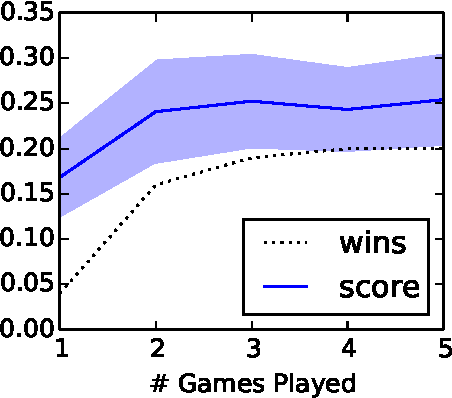
\includegraphics[scale=.61]{includes/learning-crop}
			\caption{Learning improvement on \textit{bait}}
			\label{fig:learning-results}
		\end{center}
	\end{minipage}
	\hfill
	\begin{minipage}{.45\textwidth}
		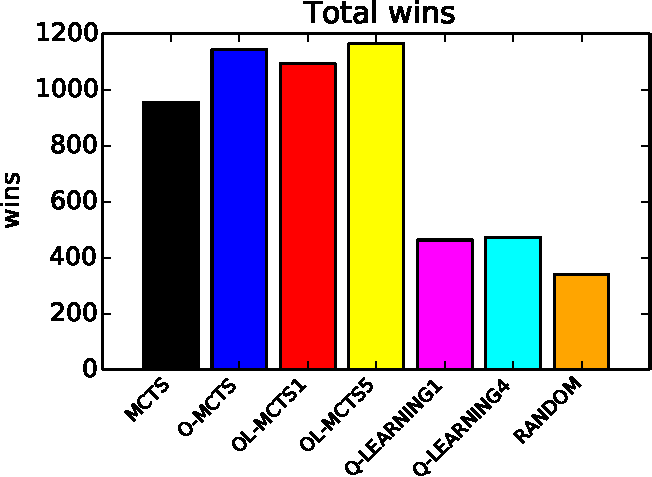
\includegraphics[width=\textwidth]{includes/totalsThesis-crop}
		\caption{Sum of all wins of each algorithm.}
		\label{fig:total-results}
	\end{minipage}
	\hfill
\end{figure}

Figure \ref{fig:total-results} shows the sum of wins over all games, all levels.
It shows a significant ($p < 0.05$) improvement of O-MCTS and OL-MCTS over MCTS.
There is no significant difference in performance of OL-MCTS over O-MCTS,
although our results suggest that it does improve for a subset of the games.
SMDP Q-learning was not proven to be useful for general video game playing, and
scores marginally better than the random algorithm. This might be a result of
the rules of the GVGAI competition, which indirectly prevent the algorithm to
learn for more than four games, which is a relatively low amount for a learning
algorithm.

Summarizing, our tests indicate that on complex games O-MCTS outperforms MCTS.
For other games it performs at least as well, as long as the number of game
sprites is not too high.  The OL-MCTS algorithm can increase performance for
some of the games, such as \textit{bait} and \textit{plaque attack}. On other
games, little to no increased perfromance can be found. 
